% RESULTS -- all values via generated tables (\input) or headline macros.
\section{Results}
\label{sec:results}

\subsection{Main benchmark}
Table~\ref{tab:main} reports the headline metrics on the $\NTest$ test
questions under the frozen shared-pool protocol (SP$_{\text{macro}}$,
SP$_{\text{micro}}$, gold-only SP$_{\text{gold}}$) alongside the
judge-free metrics (EM, $F_1$) and calibration (ECE).  Vanilla generation
without retrieval is the floor on factual support
(SP$_{\text{macro}}{=}\SPVanilla$); always-on RAG retrieves for every
question and is the strongest system on this benchmark
(SP$_{\text{macro}}{=}\SPRAG$, EM $\EMRAG$); CoVe verifies but
regenerates wholesale, landing between them on support
(SP$_{\text{macro}}{=}\SPCoVe$).  HealGen's localized repair attains
SP$_{\text{macro}}{=}\SPHealGen$ with a mean of \RetrHealGen{} retrieval
calls per question and mean latency \LatHealGen{}s on CPU
(Table~\ref{tab:efficiency}).  On SP$_{\text{macro}}$, HealGen is
significantly above vanilla ($\Delta{=}\DeltaHealVanilla$, Holm
$p{<}.001$), significantly below RAG ($\Delta{=}\DeltaHealRAG$, Holm
$p{<}.001$), and not resolved against CoVe ($\Delta{=}\DeltaHealCoVe$,
Holm $p{=}\PHolmCoVe$) --- the last comparison is uninformative at
$N{=}\NTest$, not
evidence of equivalence.

\begin{table*}[t]
\centering
\caption{Main benchmark on $\NTest$ HaluEval-QA test questions, shared
\texttt{flan-t5-base} generator, frozen shared-pool scoring (SP columns)
plus the gold-only condition (SP$_{\text{gold}}$; judge credits only the
gold passage).  95\% CIs are paired bootstrap over questions (2000
resamples).}
\label{tab:main}
% Auto-generated by make_tables.py from results/system_summary.csv
\begin{tabular}{l c c c c c c c c}
\toprule
System & SP$_{macro}$ [95\% CI] & SP$_{micro}$ & SP$_{gold}$ & HR & Any-HR & EM & F1 & ECE \\
\midrule
Vanilla & 0.6067 [0.5333, 0.6867] & 0.6067 & 0.26 & 0.3933 & 0.3933 & 0.14 & 0.1935 & 0.1213 \\
RAG & 0.9933 [0.98, 1.0] & 0.9933 & 0.9133 & 0.0067 & 0.0067 & 0.7733 & 0.8413 & 0.0164 \\
CoVe & 0.8667 [0.8133, 0.92] & 0.8667 & 0.3533 & 0.1333 & 0.1333 & 0.1867 & 0.2295 & 0.0598 \\
\textbf{HealGen} & 0.82 [0.76, 0.88] & 0.8269 & 0.3067 & 0.1731 & 0.18 & 0.14 & 0.1877 & 0.0402 \\
\bottomrule
\end{tabular}

\end{table*}

\begin{table}[t]
\centering
\caption{Efficiency: mean BM25 calls per question, end-to-end latency on
CPU (mean / p50 / p95), and abstention rate.}
\label{tab:efficiency}
\resizebox{\columnwidth}{!}{% Auto-generated by make_tables.py from results/system_summary.csv
\begin{tabular}{l c c c c c}
\toprule
System & BM25 calls (mean) & Lat. mean (s) & Lat. p50 (s) & Lat. p95 (s) & Abst. \\
\midrule
Vanilla & 0.0 & 0.59 & 0.52 & 1.01 & 0.0 \\
RAG & 1.0 & 1.53 & 0.99 & 6.03 & 0.0 \\
CoVe & 1.0 & 7.8 & 8.2 & 20.67 & 0.0 \\
\textbf{HealGen} & 1.0 & 8.18 & 8.54 & 15.16 & 0.0 \\
\bottomrule
\end{tabular}
}
\end{table}

\paragraph{Gold-only condition.}
The SP$_{\text{gold}}$ columns (Table~\ref{tab:main}) score every
emitted claim against the gold passage alone, removing retrieval-overlap
credit.  The condition separates the systems sharply: RAG keeps almost
all of its support ($\SPGoldRAG$ of its shared-pool SP survives), while
CoVe ($\SPGoldCoVe$), HealGen ($\SPGoldHealGen$), and vanilla
($\SPGoldVanilla$) drop to the bottom third.  This is the expected
signature of each system's answer style on this benchmark --- RAG
extracts the retrieved (usually gold) passage nearly verbatim, so its
claims match gold under the lexical branch, whereas HealGen's localized
repair rephrases claims into hedge or summary form that the same lexical
branch does not credit against gold alone.  Read together, the two
conditions say: HealGen's support under SP$_{\text{macro}}$ is real but
partly retrieval-overlap-mediated, and its repair output is more
abstractive than RAG's extractive answers --- a difference the
judge-free EM/$F_1$ columns show from the other side (RAG's extraction
also matches the short gold answer best).

\subsection{Significance}
Table~\ref{tab:pairwise} gives paired bootstrap tests on
SP$_{\text{macro}}$ with Holm--Bonferroni correction over the six
comparisons.  Five of six resolve: RAG is significantly above every
other system (all Holm $p{<}.001$), both CoVe and HealGen are
significantly above vanilla, and HealGen's deficit to RAG is
significant (all Holm $p{<}.001$).  The one
unresolved comparison is HealGen vs.\ CoVe ($\Delta{=}\DeltaHealCoVe$,
Holm $p{=}\PHolmCoVe$): its paired confidence interval includes zero
(Table~\ref{tab:pairwise}), and at $N{=}\NTest$ the test is underpowered
for a gap of this size, so we report it as ``not resolved'' rather
than as a tie.

\begin{table}[t]
\centering
\caption{Pairwise tests on SP$_{\text{macro}}$: $\Delta$ with 95\%
paired-bootstrap CI (2000 resamples), Holm-corrected over 6
comparisons; $^{*}$ marks Holm $p<.05$.}
\label{tab:pairwise}
\resizebox{\columnwidth}{!}{% Auto-generated by make_tables.py from results/pairwise_tests.csv
\begin{tabular}{l c c c}
\toprule
Comparison ($SP_{macro}$) & $\Delta$ & raw $p$ & Holm $p$ \\
\midrule
HealGen vs Vanilla & 0.213 & $<.001$ & $<.001$$^{*}$ \\
HealGen vs RAG & -0.173 & $<.001$ & $<.001$$^{*}$ \\
HealGen vs CoVe & -0.047 & 0.203 & 0.203 \\
CoVe vs RAG & -0.127 & $<.001$ & $<.001$$^{*}$ \\
CoVe vs Vanilla & 0.260 & $<.001$ & $<.001$$^{*}$ \\
RAG vs Vanilla & 0.387 & $<.001$ & $<.001$$^{*}$ \\
\bottomrule
\end{tabular}
}
\end{table}

\subsection{Ablations}
Table~\ref{tab:ablation} removes one HealGen component at a time on the
same questions, judged against the same frozen pools as the main systems
(paired fairness).  The result is asymmetric and, in light of
\S\ref{sec:limitations}, expected: disabling CRE (uniform risk $1.0$)
or AESP (always-retrieve) reproduces the full system \emph{exactly} ---
SP$_{\text{macro}}$, Any-HR, EM, $F_1$, and retrieval calls are
identical row-for-row --- because on this benchmark both components
already fire uniformly (every draft claim exceeds the risk threshold,
every claim starts against an empty pool).  Disabling LSHE, by contrast,
costs \SPDropLSHE{} SP$_{\text{macro}}$
($\SPHealGen \rightarrow \SPNoLSHE$) and more
than doubles Any-HR ($\AnyHRHealGen \rightarrow \AnyHRNoLSHE$) at
unchanged EM, near-identical $F_1$ (Table~\ref{tab:ablation}), and
identical retrieval cost: localized repair is
the only component
whose contribution this benchmark can measure, and it acts purely by
making claims more supportable, not by making answers more
gold-exact.

\begin{table}[t]
\centering
\caption{Ablations on the same $\NTest$ questions and frozen pools.
Any-HR is the fraction of answers with at least one unsupported claim.}
\label{tab:ablation}
\resizebox{\columnwidth}{!}{% Auto-generated by make_tables.py from results/ablations.csv + results/main.csv
\begin{tabular}{l c c c c c}
\toprule
Variant & SP$_{macro}$ & Any-HR & EM & F1 & BM25 calls \\
\midrule
\textbf{HealGen (full)} & 0.820 & 0.180 & 0.140 & 0.188 & 1.0 \\
w/o CRE (uniform risk) & 0.820 & 0.180 & 0.140 & 0.188 & 1.0 \\
w/o AESP (always retrieve) & 0.820 & 0.180 & 0.140 & 0.188 & 1.0 \\
w/o LSHE (hedge only) & 0.620 & 0.380 & 0.140 & 0.189 & 1.0 \\
\bottomrule
\end{tabular}
}
\end{table}

\subsection{Judge gate and threshold sensitivity}
Table~\ref{tab:judge-validation} is the pre-registered judge gate
measured before any benchmark run (contrast pairs, seed 44); it passed
and the primary judge was then frozen.  Table~\ref{tab:tau} shows the
full dev-split sweep run after the fact; the committed test runs used
$\tau{=}0.7$ frozen from an earlier partial sweep --- a discrepancy
that is provably inert on this benchmark and is disclosed in
\S\ref{sec:method} and \S\ref{sec:limitations}.

\begin{table}[t]
\centering
\caption{Judge validation gate on 100 labeled contrast pairs (gold vs.\
hallucinated answers), measured at $T{=}1$ before the benchmark ran.}
\label{tab:judge-validation}
\resizebox{\columnwidth}{!}{% Auto-generated by make_tables.py from results/judge_validation.csv
\begin{tabular}{l l c c c}
\toprule
Role & Model & Accuracy & AUC & $n$ \\
\midrule
Primary & DeBERTa-v3-base-mnli-fever-anli & 0.83 & 0.9895 & 200 \\
Secondary & nli-deberta-v3-small & 0.85 & 0.9877999999999999 & 200 \\
\bottomrule
\end{tabular}
}
\end{table}

\begin{table}[t]
\centering
\caption{AESP sufficiency-threshold sensitivity on the 50-question dev
split (F1 over the candidate grid).}
\label{tab:tau}
% Auto-generated by make_tables.py from results/tau_sensitivity.csv
\begin{tabular}{c c c c c c}
\toprule
$\tau$ & Precision & Recall & F1 & Accuracy & Selected \\
\midrule
0.3 & 0.5556 & 0.597 & 0.5755 & 0.6169 & True \\
0.5 & 0.5106 & 0.3582 & 0.4211 & 0.5714 & False \\
0.7 & 0.4545 & 0.0746 & 0.1282 & 0.5584 & False \\
\bottomrule
\end{tabular}

\end{table}

\subsection{Calibration and diagnostics}
Figure~\ref{fig:reliability} plots the reliability diagram of recorded
confidences against frozen-pool support verdicts; the ECE column of
Table~\ref{tab:main} summarizes it (unfitted confidences, see
Limitations).  Figure~\ref{fig:efficiency} shows the support/latency and
support/retrieval trade-off per system.

\begin{figure}[t]
\centering
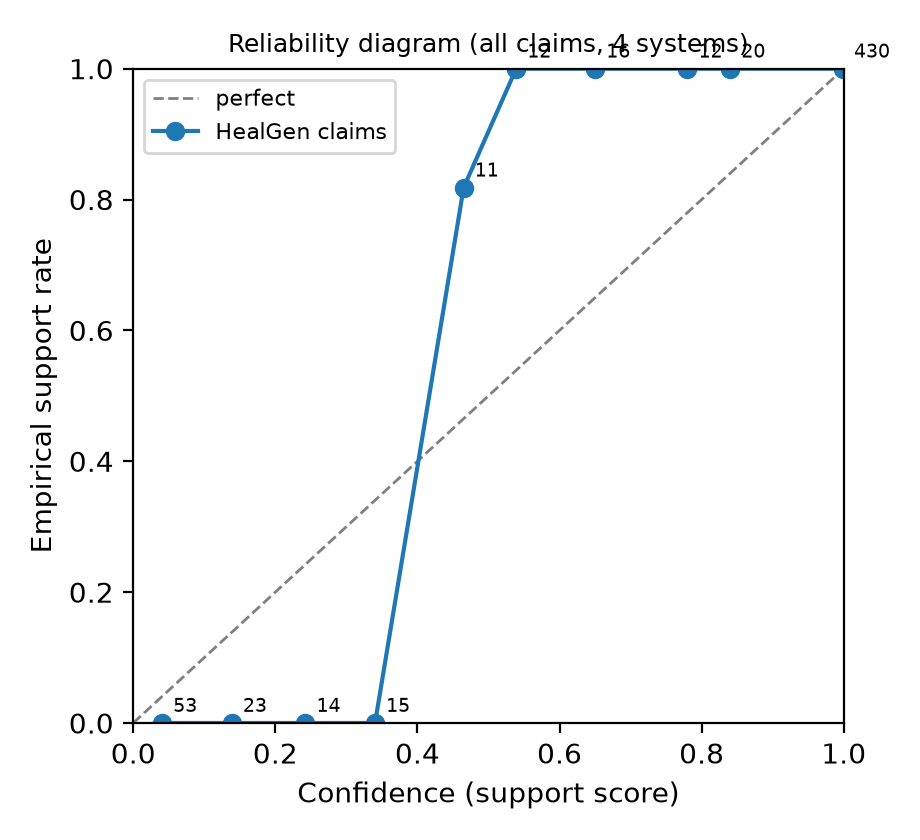
\includegraphics[width=\columnwidth]{figures/reliability_diagram.png}
\caption{Reliability diagram: recorded confidence vs.\ frozen-pool
support frequency (10 bins) over all emitted claims.}
\label{fig:reliability}
\end{figure}

\begin{figure}[t]
\centering
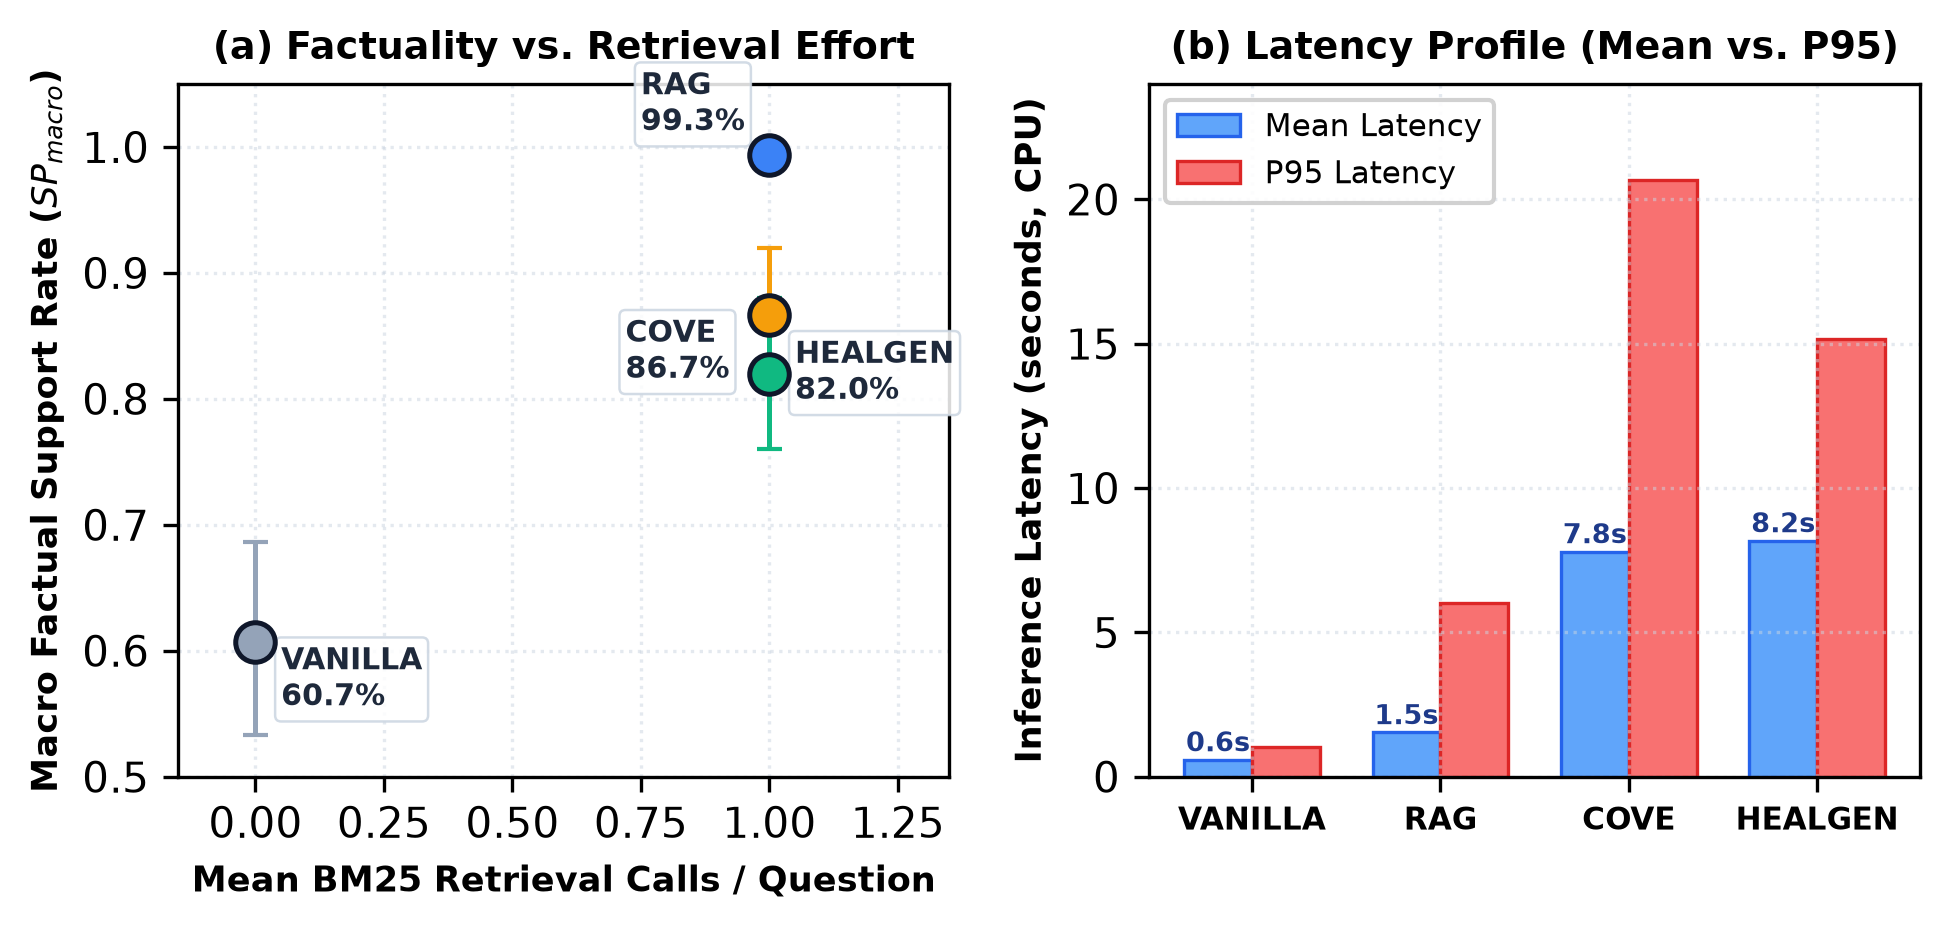
\includegraphics[width=\columnwidth]{figures/latency_retrieval.png}
\caption{Cost side of the ledger: end-to-end latency and retrieval calls
per system against factual support.}
\label{fig:efficiency}
\end{figure}
